\documentclass[12pt,twoside]{article}   
\usepackage{light}

\hidesolutions
%\showsolutions

\newcommand{\hint}[1]{({\it Hint: #1})}
\newcommand{\card}[1]{\left|#1\right|}

\begin{document}
\problemset{6}{October 7, 2014}{Monday, October 13}
\noindent \textbf{Reading Assignment:}   Sections 7.1-7.9
\\

%%%%%%%%%%%%%%%%%%%%%%%%%%%%%%%%%%%%%%%%%%%%%%%%%%%%%%%%%%%%%%%%%%%%%%%%%%%%%%%

\begin{problem}{20}
    The adjacency matrix $A$ of a graph $G$ with $n$ vertices as defined in lecture is an $n \times n$
    matrix in which $A_{i,j}$ is 1 if there is an edge from $i$ to $j$ and 0 if there is not.
    In lecture we saw how 
    the smallest $k$ where $A^k_{i,j} \neq 0$ describes the length
    of the shortest path from $i$ to $j$. Given a combinatorial interpretation of the following statements about the adjacency matrix in terms of connectivity properties of $G$. For example, the smallest $k$ such that $A^k_{i,j}$ is non-zero means that the distance from $i$ to $j$ is at most $k$. 
\bparts
\ppart{5}
    The smallest $k$ such that for every pair $(i,j)$ at least one of
    $A_{i,j}, A_{i,j}^2, \dots , A^k_{i,j}$ is non-zero.
    \solution{
        This is the diameter of the graph. It is the smallest $k$ for which
        there exists a path of length less than or equal to $k$ for every
        pair of vertices.
    }

\ppart{5}
    $\forall k. A^{k}_{i,j} = 0$
    \solution{
        There is no path in $G$ from $i$ to $j$.
    }

\ppart{5}
    $\forall i \forall k. A^{k}_{i,i} = 0$
    \solution{
        The graph is acyclic. 
    }

\ppart{5}
$\forall k$, we can write $A^k$ as $\left[ \begin{array}{cc}
                                            X & 0 \\
                                            0 & Y 
                                    \end{array} \right]$
    \solution{
    There is no path from $X$ to $Y$ and so there are at least two connected components.
    }

\eparts
\end{problem}


\begin{problem}{15}
A set of PageRank values is stationary if the amount of PageRank
 going into each vertex is the same
as the amount leaving the vertex on every update.
Prove that a strongly connected graph has at most one set of PageRank values that are stationary. There always is a set of PageRank values that are stationary, but
we are not asking you prove this.

\bparts

\ppart{7}
  For two sets of values of PageRank, $d_1$ and $d_2$, let $\gamma$ be defined as 
  $\gamma \eqdef \max_{x \in V} \frac{d_1(x)}{d_2(x)}$, the maximum ratio
  of a value in $d_1$ over the corresponding value in $d_2$.
  Show that there exists a directed edge from $y$ to $z$ such that
  $d_1(y)/d_2(y) < \gamma$ and $d_1(z)/d_2(z) = \gamma$.

\solution{
  $\gamma$ must be attained at some vertex and not all vertices have 
  a ratio of $\gamma$ because if they did then the
values would be the same.
  Because the graph is strongly connected, we can follow edges backwards until we 
  arrive at any other vertex and there must be some
  vertex along the way that does not attain $\gamma$.
  So such an edge must exist.
}

\ppart{8}
  Prove that a strongly connected graph has at most one set of PageRank
values that are stationary by deriving a contradiction using the edge
  found in part a.

\solution{
  Assume for the sake of contradiction that there are two stationary
values $d_1$ and $d_2$.  Let $\gamma$ be defined as 
  $\gamma \eqdef \max_{x \in V} \frac{d_1(x)}{d_2(x)}$, the maximum ratio
  of a value in $d_1$ over the corresponding value in $d_2$.

  Pick an edge from $y$ to $z$ such that
  $d_1(y)/d_2(y) < \gamma$ and $d_1(z)/d_2(z) = \gamma$.
  $\gamma$ must be attained at some vertex and not all vertices have 
  a ratio of $\gamma$ because if they did then the
values would be the same.
  Because the graph is strongly connected, we can follow edges until we 
  arrive at any other vertex and there must be some
  vertex along the way that does not attain $\gamma$.
  So such an edge must exist.

  Define $p(x,z)$ to be $\frac{\text{Number of edges from x to z}}{\text{Number of edges out of x}}$
  We apply one step of PageRank to $d_1$ and $d_2$ which are stationary values $\widehat{d_1}$ and $\widehat{d_2}$.
  \begin{equation}\label{d1}
    d_1(z) = \widehat{d_1}(z) = \sum_{x: x\rightarrow z} d_1(x) p(x,z),
  \end{equation}
  and
  \begin{equation}\label{d2}
    d_2(z) = \widehat{d_2}(z) = \sum_{x: x\rightarrow z} d_2(x) p(x,z).
  \end{equation}

  Substituting $d_1(z) = \gamma d_2(z)$ into \eqref{d1}, and recalling
  that $d_1(x) \leq \gamma d_2(x)$ for all $x$, we have
  \begin{align*}
    \gamma d_2(z)
        &= \sum_{x: x\rightarrow z} d_1(x) p(x,z) \\
        &= \paren{\sum_{x \neq y: x\rightarrow z}
          d_1(x)p(x,z)} + d_1(y) p(y,z) \\
        &\leq \paren{\sum_{x \neq y: x\rightarrow z} \gamma d_2(x)
          p(x,z)} + d_1(y) p(y,z) \\
        &\leq \paren{\paren{\gamma \sum_{x: x\rightarrow z} d_2(x)
          p(x,z)} - \gamma d_2(y)p(y,z)} + d_1(y) p(y,z) \\
        &\leq \gamma d_2(z) - \gamma d_2(y)p(y,z) + d_1(y) p(y,z)\\
        &< \gamma d_2(z) - \gamma d_2(y)p(y,z) + \gamma d_2(y) p(y,z)\\
        &< \gamma d_2(z).
  \end{align*}
  The strict inequality at the next to last step of the derivation
  follows from the assumption that $d_1(y) < \gamma d_2(y)$, and
  $p(y,z) > 0$.  Thus, we have shown $d_2(z) < d_2(z)$, which is a
  contradiction.
}

\eparts
\end{problem}


%%%%%%%%%%%%%%%%%%%%%%%%%%%%%%%%%%%%%%%%%%%%%%%%%%%%%%%%%%%%5555


\begin{problem}{15} 

\bparts

\ppart{5}
    For the graph in Figure~\ref{scc-graph}, compute the first two iterations
    of PageRank, starting from uniform PageRank values across all vertices.

    \begin{figure}[h!]
    \begin{center}
        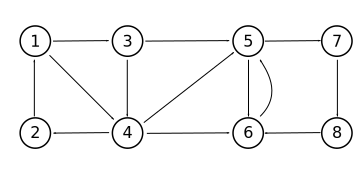
\includegraphics{ps6-scc-graph.pdf}
        \caption{A graph of web pages and links.}
        \label{scc-graph}
    \end{center}
    \end{figure}

    \solution{
        In the table below, we write the PageRank value of each vertex at
        iterations $0$, $1$, and $2$. We also include, for each vertex, the
        individual contributions made to that vertex in computing the next
        stage, which are summed in computing the following PageRank value.

        \begin{center}
        \begin{tabular}{r|cccccccc}
            & 1 & 2 & 3 & 4 & 5 & 6 & 7 & 8 \\
            \hline \\[-0.5em]
            iter 0  & $\frac18$ & $\frac18$ & $\frac18$ & $\frac18$ & $\frac18$ & $\frac18$ & $\frac18$ & $\frac18$ \\[1em]
            contrib & $\frac18$ & $\frac1{24}$ & $\frac1{16}$ & $\frac1{16}, \frac18$ & $\frac18, \frac1{16}, \frac1{24}$ & $\frac18, \frac1{16}, \frac1{24}$ & $\frac1{16}$ & $\frac18$ \\[1em]
            iter 1  & $\frac18$ & $\frac1{24}$ & $\frac1{16}$ & $\frac18$ & $\frac{11}{48}$ & $\frac{11}{48}$ & $\frac1{16}$ & $\frac18$ \\[1em]
            contrib & $\frac1{24}$ & $\frac1{24}$ & $\frac1{16}$ & $\frac1{16}, \frac1{32}$ & $\frac1{24}, \frac1{32}, \frac{11}{48}$ & $\frac18, \frac1{24}, \frac{11}{96}$ & $\frac{11}{96}$ & $\frac1{16}$ \\[1em]
            iter 2  & $\frac1{24}$ & $\frac1{24}$ & $\frac1{16}$ & $\frac3{32}$ & $\frac{29}{96}$ & $\frac{9}{32}$ & $\frac{11}{96}$ & $\frac1{16}$ 
        \end{tabular}
        \end{center}
    }

\ppart{10}
    A strongly connected component of a directed graph is a subgraph which
    has the property that for every pair of vertices 
    $u$ and $v$, there exists a path from
    $u$ to $v$ and one from $v$ to $u$. Also, every vertex which can be
    reached by a path starting in the strongly connected component is also
    in the strongly connected component.
    Suppose that a graph $G$ consists of exactly two strongly connected
    components $C_1$ and $C_2$, and that there exist edges from $C_1$ to
    $C_2$ (but not from $C_2$ to $C_1$). There is always a stationary set of
    values which is non-negative. Prove that the stationary PageRank 
    values of this graph are entirely concentrated in $C_2$, i.e.\ that the
    PageRank values are all zero on $C_1$.

    \solution{
        For any vertex $v$, let $p(v)$ denote the stationary PageRank value
        at $v$, so that if we apply another step of the PageRank update rule
        to these values, they remain unchanged.  Suppose for a contradiction
        that for some vertex $v \in C_1$, $p(v) \neq 0$.

        Let $w$ be any other vertex of $C_1$; we first claim that the PageRank
        value at $w$ is positive. From the hypothesis that $C_1$ is strongly
        connected, there exists a path from $v$ to $w$, of some length $k$. If
        we were to apply $k$ steps of the PageRank algorithm, then
        the non-zero PageRank value $p(v)$ would yield some positive
        contribution to the resulting value at $w$, via the path mentioned
        above. The resulting PageRank value at $w$ after $k$ steps would then
        be positive. As the PageRank values were already stationary we
        can conclude that $p(w) > 0$.

        Now, we know that some vertex $w \in C_1$ has an edge leading into
        $C_2$. As the PageRank value $p(w)$ is positive, then if we were to
        apply another step of the PageRank update rule, vertex $w$ would make
        a contribution of at least $\frac{p(w)}{\mathrm{outdeg}(w)}$ to the
        total PageRank of component $C_2$. There are however no edges from
        $C_2$ to $C_1$. As the total PageRank in a graph always sums to $1$,
        we must conclude that the total PageRank in component $C_1$ decreases
        by at least $\frac{p(w)}{\mathrm{outdeg}(w)} > 0$ by applying the
        update rule.

        But these PageRank values were assumed to be stationary, and we
        have argued above that they must change when we apply the update step.
        This is a contradiction, and so the stationary PageRank values must
        be zero throughout component $C_1$, as desired.
    }

\eparts

\end{problem}



%-----------------------------------------------------------------%
% source: Velleman 4.6, Exercise 3.
% topic: equivalence relations
% last used Fall00 Problem Set 3 (in ProblemRepository)

% In 2010 and 2012

\begin{problem}{20}
For each of the following, either prove that it is an equivalence relation and state its equivalence classes, or give an example of why it is not an equivalence relation. 

\bparts
\ppart{5}
$R_n := \{(x, y) \in \mathbb Z \times \mathbb Z \textrm{ s.t. } x \equiv y \pmod n \}$
\solution{
	It is an equivalence relation.  To prove this, we will show that $R_n$ is symmetric, transitive, and reflexive.
	\begin{itemize}
		\item
			\textbf{Reflexive}: $x \equiv x \pmod n$.  This is because $x = x + 0 \cdot n$.  
		\item 
			\textbf{Symmetric}: We want to show that $R_n(x, y) \Rightarrow R_n(y, x)$.  If $R_n(x, y)$, then there is some $c \in \mathbb Z$ such that $x = y + c \cdot n$.  But then,
				subtracting $c \cdot n$ from both sides, we have that $y = x + (-c) \cdot n$, so $y \equiv x \pmod n$.  So $R_n(y, x)$, and the symmetric property holds.
		
		\item
			\textbf{Transitivity}.  Suppose $R_n(x, y)$ and $R_n(y, z)$.  From the first statement, we know that there is some $c \in \mathbb Z$ such that $x = y + c\cdot n$.  From the second,
			we know that there is some $d \in \mathbb Z$ such that $y = z + d \cdot n$.  Substituting in this value of y, we see that $x = (z + d \cdot n) + c \cdot n = z + (d + c) \cdot n$.  The
			sum $c + d$ is an integer, so $R_n(x, z)$ holds.  
	\end{itemize}
	The equivalence classes are then the sets of numbers congruent to the numbers $\{0, 1, \ldots, n-1 \}$ modulo n.
}

\ppart{5}
$R := \{ (x, y) \in P \times P \textrm{ s.t. } x \textrm{ is taller than } y \}$
where $P$ is the set of all people in the world today.
\solution{
	This is not an equivalence relation, because the concept of symmetry is broken.  If $y$ is taller than $x$, then $x$ is not taller than $y$.
}

\ppart{5} 
$R := \{ (x, y) \in \mathbb Z \times \mathbb Z \textrm{ s.t. } gcd(x,y)=1 \}$
\solution{
	This is not an equivalence relation, because transitivity is broken.  Consider the case when $x = 3$, $y = 7$, and $z = 15$.  Then, $gcd(x,y)=1$ and $gcd(y,z)=1$, but $gcd(x,z)=3\neq 1$.
}

\ppart{5}
$R_G := $ the set of $(x, y) \in V \times V$ such that $V$ is the set of vertices of a graph $G$, and there is a path $x, v_1, \ldots, v_k, y$ from $x$ to $y$ along the edges of $G$.

\solution{
	This is an equivalence relation.  We will show this by proving that it obeys reflexivity, symmetry, and transitivity.
	\begin{itemize}
	\item
		\textbf{Reflexivity}: Any vertex is connected to itself.  
	\item
		\textbf{Symmetry}: If $R_G(x, y)$, then there is a path $x, v_1, \ldots, v_k, y$ from $x$ to $y$.  The reverse of this path is $y, v_k, \ldots, v_1, x$, and is a path from
		$y$ to $x$.  So $R_G(y, x)$.
	\item
		\textbf{Transitivity}:  Suppose $R_G(x, y)$ and $R_G(y, z)$.  Then, there is a path from $x$ to $y$: $x, v_1, \ldots, v_k, y$.  Furthermore, there is a path from $y$ to $z$: 
		$y, w_1, \ldots, w_l, z$.  But then, the concatenation of those two is a path $x, v_1, \ldots, v_k, y, w_1, \ldots, w_l, z$ from $x$ to $z$.  So $R_G(x, z)$.
	\end{itemize}
	
	Thus we have shown that $R_G$ is an equivalence relation on a graph $G$, and the equivalence classes are the connected components of $G$.
}

\eparts
\end{problem}


%%%%%%%%%%%%%%%%%%%%%%%%%%%%%%%%%%%%%%%%%%%%%%%%%%%%%%%%%%%%%%%%%%%%%%%%%%%%%%


\begin{problem}{10}
Let $R_1$ and $R_2$ be two equivalence relations on a set, $A$.  Prove
or give a counterexample to the claims that the following are also
equivalence relations:

\bparts

\ppart{5} 
$R_1 \intersect R_2$.

\solution{
Let $R \eqdef R_1 \intersect R_2$.  We give two proofs that $R$ is an
equivalence relation using different characterizations of equivalence
relations.

\begin{proof}
We first prove that $R$ is an equivalence relations by showing that $R$ is
reflexive, symmetric, and transitive.

\emph{Reflexive:} $R_i$ is reflexive because it is an equivalence
relation, for $i=1,2$.  So $(a,a) \in R_i$ for $i=1,2$ and all $a \in A$.
So, $(a,a) \in (R_1 \intersect R_2) = R$ for all $a \in A$, that is, $R$
is reflexive.

\emph{Transitive:} Suppose $(a,b), (b,c) \in R$.  Since $R = R_1
\intersect R_2$, we have $(a,b), (b,c) \in R_i$ for $i=1,2$.  But $R_i$ is
an equivalence relation, and so is transitive.  Therefore, $(a,c) \in
R_i$, and so $(a,c) \in R_1\intersect R_2 = R$.  This shows that $R$ is
transitive.

\emph{Symmetric:} The proof that $R$ is symmetric follows the same format.

\end{proof}

\begin{proof}
Since $R_i$ is an equivalence relation for $i=1,2$, there is by
definition a total function, $f_i$, with domain, $A$, such that
\[
aR_i b \quad\text{ iff }\quad f_i(a) = f_i(b).
\]
Define the function, $f$, with domain, $A$, by
\[
f(a) \eqdef (f_1(a),f_2(a)).
\]
Clearly $f$ is total, since $f_i$ is total for $i=1,2$.  Now we have,
\begin{align*}
aRb \quad &  \text{ iff }\quad a(R_1 \intersect R_2)b & \text{def.\ of $R$}\\
    &  \text{ iff }\quad aR_ib\text{ for }i=1,2 & \text{def.\ of $\intersect$}\\
    &  \text{ iff }\quad f_i(a)=f_i(b) \text{ for }i=1,2 & \text{def.\ of $f_i$}\\
    &  \text{ iff }\quad (f_1(a),f_2(a)) = (f_1(b),f_2(b)) & \text{def.\ of $=$ pairs}\\
    &  \text{ iff }\quad f(a) = f(b) & \text{def.\ of $f$}.
\end{align*}
That is
\[
aRb \quad \text{ iff }\quad f(a) = f(b),
\]
which proves that $R$ is the equivalence relation $\equiv_f$.
\end{proof}
}


\ppart{5}
$R_1 \union R_2$.

\solution{
We give a counterexample showing that $R_1 \union R_2$ may not be
an equivalence relation.  Let $R_1$ and $R_2$ be the relations on
$\set{1, 2, 3}$ where
\begin{align*}
R_1 \eqdef & \set{(1,1) (2,2) (3,3) (1,2) (2,1)},\\
R_2 \eqdef & \set{(1,1) (2,2) (3,3) (2,3) (3,2)}.
\end{align*}
It's easy to check that $R_1$ and $R_2$ are both equivalence relations.
But $R_1\union R_2$ is not transitive, because $(1,2),(2,3) \in R_1\union R_2$
and $(1,3) \notin R_1\union R_2$.  Therefore $R_1\union R_2$ is not an
equivalence relation.
}

\eparts

\end{problem}


%%%%%%%%%%%%%%%%%%%%%%%%%%%%%%%%%%%%%%%%%%%%%%%%%%%%%%%%%%%%%%%%%%%%%%%%5


\begin{problem}{15}
In this problem we study partial orders (posets). Recall that a weak partial order $\preceq$ on a set $X$ is reflexive $(x \preceq x)$, anti-symmetric ($x \preceq y \wedge y \preceq x \rightarrow x = y$), and transitive ($x \preceq y \wedge y \preceq z \rightarrow x \preceq z$). Note that it may be the case that neither $x \preceq y$ nor $y \preceq x$. A chain is a list of {\it distinct} elements $x_1, \ldots, x_i$ in $X$ for which $x_1 \preceq x_2 \preceq \cdots \preceq x_i$. An antichain is a subset $S$ of $X$ such that for all distinct $x, y \in S$, neither $x \preceq y$ nor $y \preceq x$. 

The aim of this problem is to show that any sequence of $(n-1)(m-1) + 1$ integers either contains a non-decreasing subsequence of length $n$ or a decreasing subsequence of length $m$. Note that the given sequence may be out of order, so, for instance, it may have the form $1, 5, 3, 2, 4$ if $n = m = 3$. In this case the longest non-decreasing and longest decreasing subsequences have length $3$ (for instance, consider $1, 2, 4$ and $5, 3, 2$).

%\solution{Consider the set $S_1$ of all minimal elements $x \in X$. Then $S_1$ is an antichain since for distinct $x,y \in S_1$, neither $x \preceq y$ nor $y \preceq x$ since both $x$ and $y$ are minimal. Now let $S_2$ be the set of all minimal elements in $X \setminus S_1$. Then $S_2$ is also an antichain. We repeat this process, obtaining sets $S_1, \ldots, S_r$ for which, (1) for all $1 \preceq i \preceq r$, $S_i$ is an antichain, (2) $S_i \cap S_j = \emptyset$ for all $i \neq j$, and (3) $X = S_1 \cup S_2 \cup \cdots \cup S_r$. Thus, $S_1, \ldots, S_r$ are antichains that partition $X$.

%It remains to show that we can choose $r \geq n$. We know that $X$ contains a chain of $n$ elements, i.e., $n$ distinct elements $x_1 \preceq x_2 \preceq \cdots \preceq x_n$. Then, for every $i$, $S_i$ can contain at most one $x_j$, since if $x_j$ and $x_{j'}$ were in $S_i$ for some $j < j'$, by transitivity of a poset, $x_j \preceq x_{j'}$, contradicting the fact that $S_i$ is an antichain. It follows that $r \geq n$.}

%Now we show $r \leq n$. Consider any element $s_r \in S_r$. Then we must have $s_{r-1} \preceq s_r$ for some element $s_{r-1} \in S_{r-1}$, as otherwise we would have put $s_{r}$ in $S_{r-1}$. Similarly, there must be some element $s_{r-2} \in S_{r-2}$ for which $s_{r-2} \preceq s_{r-1}$, as otherwise we would have put $s_{r-1}$ in $S_{r-2}$. Since $S_i \cap S_j = \emptyset$ for $i \neq j$, we obtain a list of distinct elements $s_1 \preceq s_2 \preceq \cdots \preceq s_r$, so we obtain a chain of length $r$. But the longest chain in $X$ has length $n$, so $r \leq n$.}
\bparts

\ppart{5} Label the given sequence of $(n-1)(m-1)+1$ integers $a_1, a_2, \ldots, a_{(n-1)(m-1)+1}$. Show the following relation $\preceq$ on $\{1, 2, 3, \ldots, (n-1)(m-1)+1\}$ is a weak poset: $i \preceq j$ if and only if $i\leq j$ and $a_i \leq a_j$ (as integers).

\solution{We show reflexivity, anti-symmetry, and transitivity. Clearly $i \preceq i$ since $i \leq i$ and $a_i \leq a_i$, so $\preceq$ is reflexive. Next, suppose $i \preceq j$ and $j \preceq i$. Then $i \leq j \leq i$, so $i = j$, and $\preceq$ is anti-symmetric. Finally, suppose $i \preceq j$ and $j \preceq k$. Then $i \leq j$ and $j \leq k$, so $i \leq k$. Moreover, $a_i \leq a_j$ and $a_j \leq a_k$, so $a_i \leq a_k$. Thus, $\preceq$ is transitive.}

For the next part, we will need to use Dilworth's theorem. Recall that Dilworth's theorem states that if $(X, \preceq)$ is any poset whose longest chain has length $n$, then $X$ can be partitioned into $n$ disjoint antichains. 

\ppart{5} Show that in any sequence of $(n-1)(m-1) + 1$ integers, either there is a non-decreasing subsequence of length $n$ or a decreasing subsequence of length $m$. 

\solution{Consider the $\preceq$ relation on $\{1, 2, \ldots, (n-1)(m-1)+1\}$ defined above. The length of the longest non-decreasing subsequence of the given integers is just the length of the longest chain in this poset. If the longest chain has length at least $n$, we are done, so suppose the length of the longest chain is at most $c \leq n-1$. 

Then, by the first part we know that $\{1,2, \ldots, (n-1)(m-1)+1\}$ can be decomposed into $c$ disjoint antichains. Consider the indices $i_1 \leq i_2 \leq \cdots \leq i_s$ in any antichain $A$. Then it must be the case that $a_{i_1} > a_{i_2} > \cdots > a_{i_s}$, as otherwise we would have $a_{i_j} \leq a_{i_{j'}}$ for some $j < j'$, and thus $j \preceq j'$, and $A$ could not be an antichain. It follows that there is a decreasing subsequence of length at least $|A|$.

Since it is possible to partition $\{1, 2, \ldots, (n-1)(m-1)+1\}$ into $c \leq n-1$ disjoint antichains, one such antichain must have size at least
$$\frac{(n-1)(m-1)+1}{c} \geq \frac{(n-1)(m-1)+1}{n-1} \geq m-1 + \frac{1}{n-1} \geq m,$$which completes the proof.}

\ppart{5} Construct a sequence of $(n-1)(m-1)$ integers, for arbitrary $n$ and $m$, that has no non-decreasing subsequence of length $n$ and no decreasing subsequence of length $m$. Thus in general, the result you obtained in the previous part is best-possible.

\solution{Consider the set of integers $\{1, 2, \ldots, (n-1)(m-1)\}$. For each $1 \leq i \leq n-1$, define the decreasing subsequence of length $m-1$: $$B_i = i(m-1), \ldots, (i-1)(m-1)+1.$$
Then the $B_i$ partition $\{1, 2, \ldots, (n-1)(m-1)\}$. Consider the sequence $$S = B_1 \circ B_2 \circ \cdots \circ B_{n-1}.$$ Any non-decreasing subsequence of $S$ can contain at most one integer from any single $B_i$, since the $B_i$ are decreasing subsequences. Thus, the length of the longest non-decreasing subsequence is at most $n-1$. 

Any decreasing subsequence must be entirely contained in a single $B_i$, since for $j > i$, any integer in $B_j$ is larger than any integer in $B_i$. Thus, the length of the longest decreasing subsequence is at most $m-1$.}

\eparts

\end{problem}


%%%%%%%%%%%%%%%%%%%%%%%%%%%%%%%%%%%%%%%%%%%%%%%%%%%%%%%%%%%%%%%%%%


\begin{problem}{10}
    Let the transitive closure of a graph $G$ be the digraph $G^+ = (V, E^+ )$, where:
    $$ E^+ = \{u \rightarrow v \mid \text{there is a directed path of positive length from } u \text{ to } v \text{ in } G\}.$$
    Prove that if the graph $G$ is a directed acyclic graph, then the transitive closure of $G$ is a
    strong partial order.

\solution{
    Let’s show that the transitive closure of $G$ is a strong partial order:

    \begin{itemize}
        \item Irreflexive:
            $\neg(x \prec x)$ because the transitive closure of $G$ will not contain a path from
            a vertex to itself, since $G$ is directed acyclic.
        \item Antisymmetric: 
            If $x \prec y$ then $\neg (y \prec x)$. Else if $y \prec x$ them there will be a path from
            $x$ to itself passing through $y$, but $G$ is directed acyclic.
        \item Transitive:
            If $x \prec y$ and $y \prec z$ then $x \prec z$. This is because if there is a path from $x$ to $y$ and
            a path from $y$ to $z$ then there is a path from $x$ to $z$ passing through $y$.
    \end{itemize}
}

\end{problem}


%%%%%%%%%%%%%%%%%%%%%%%%%%%%%%%%%%%%%%%%%%%%%%%%%%%%%%%%%%%%%%%%%%
\end{document}
